\documentclass{bmstu}

\newcommand{\specialcell}[2][c]{%
	\begin{tabular}[#1]{@{}c@{}}#2\end{tabular}}

\newcommand{\img}[3] {
	\begin{figure}[H]
		\center{\includegraphics[width=#1]{inc/img/#2}}
		\caption{#3}
		\label{img:#2}
	\end{figure}
	}
	
\renewcommand\labelitemi{---}
\renewcommand\labelitemii{---}

\usepackage{multirow}

\begin{document}

\makereporttitle{Информатика и системы управления}{Программное обеспечение ЭВМ и информационные технологии}{лабораторной работе №3}{Конструирование компиляторов}{Синтаксический разбор с использованием метода рекурсивного спуска}{7}{Е.~О.~Карпова/ИУ7-22М}{А.~А.~Ступников}

\chapter{Теоретический раздел}

\subsection{Равномерное распределение}
    
Говорят, что случайная величина X имеет равномерное распределение на отрезке $[a,b]$, если её функция плотности имеет вид:

\begin{equation*}
    f_X (x) =
    \begin{cases}
        \frac{1}{b-a}, x \in [a,b] \\
        0, x \notin [a, b] \\
    \end{cases}
\end{equation*}

Значения случайной величины с двух сторон ограничены и в границах интервала имеют одинаковую вероятность. В данном интервале плотность вероятности постоянна.

Функция распределения:

\begin{equation*}
F_X (x) =
    \begin{cases}
        0, x < a \\
        \frac{x - a}{b - a}, a \le x < b \\
        1, x \geq b \\
    \end{cases}
\end{equation*}

\begin{figure}[H]
    \begin{center}
    \includegraphics[width=0.5\linewidth]{inc/uni_f.png}
    \caption{Функция плотности равномерного распределения}
    \label{fig:}
    \end{center}
\end{figure}

\begin{figure}[H]
    \begin{center}
    \includegraphics[width=0.5\linewidth]{inc/uni_Fx.png}
    \caption{Функция распределения равномерного распределения}
    \label{fig:}
    \end{center}
\end{figure}

\subsection{Распределение Эрланга}

Распределение Эрланга является непрерывным распределением, ограниченным снизу. Оно представляет собой особый случай Гамма распределения, где параметр $k$ может принимать только положительные целые значения.

Функция распределения:

\begin{equation*}
F_X(x) = 1 - \sum_{i=0}^{k-1}  \frac{1}{i!} e^{-\lambda x} (\lambda x)^n
\end{equation*}
    
Плотность распределения:

\begin{equation*}
f_X(x) = \frac{\lambda^k x^{k-1} e^{-\lambda x} } {(k-1)!}
\end{equation*}

\begin{figure}[H]
    \begin{center}
    \includegraphics[width=0.5\linewidth]{inc/erlang_f.png}
    \caption{Функция плотности распределения Эрланга}
    \label{fig:}
    \end{center}
\end{figure}

\begin{figure}[H]
    \begin{center}
    \includegraphics[width=0.5\linewidth]{inc/erlang_Fx.png}
    \caption{Функция распределения распределения Эрланга}
    \label{fig:}
    \end{center}
\end{figure}
\chapter{Практический раздел}

На рисунках~\ref{fig:1}--\ref{fig:2} представлена работа разработанной программы.

\begin{figure}[ht]
    \centering
    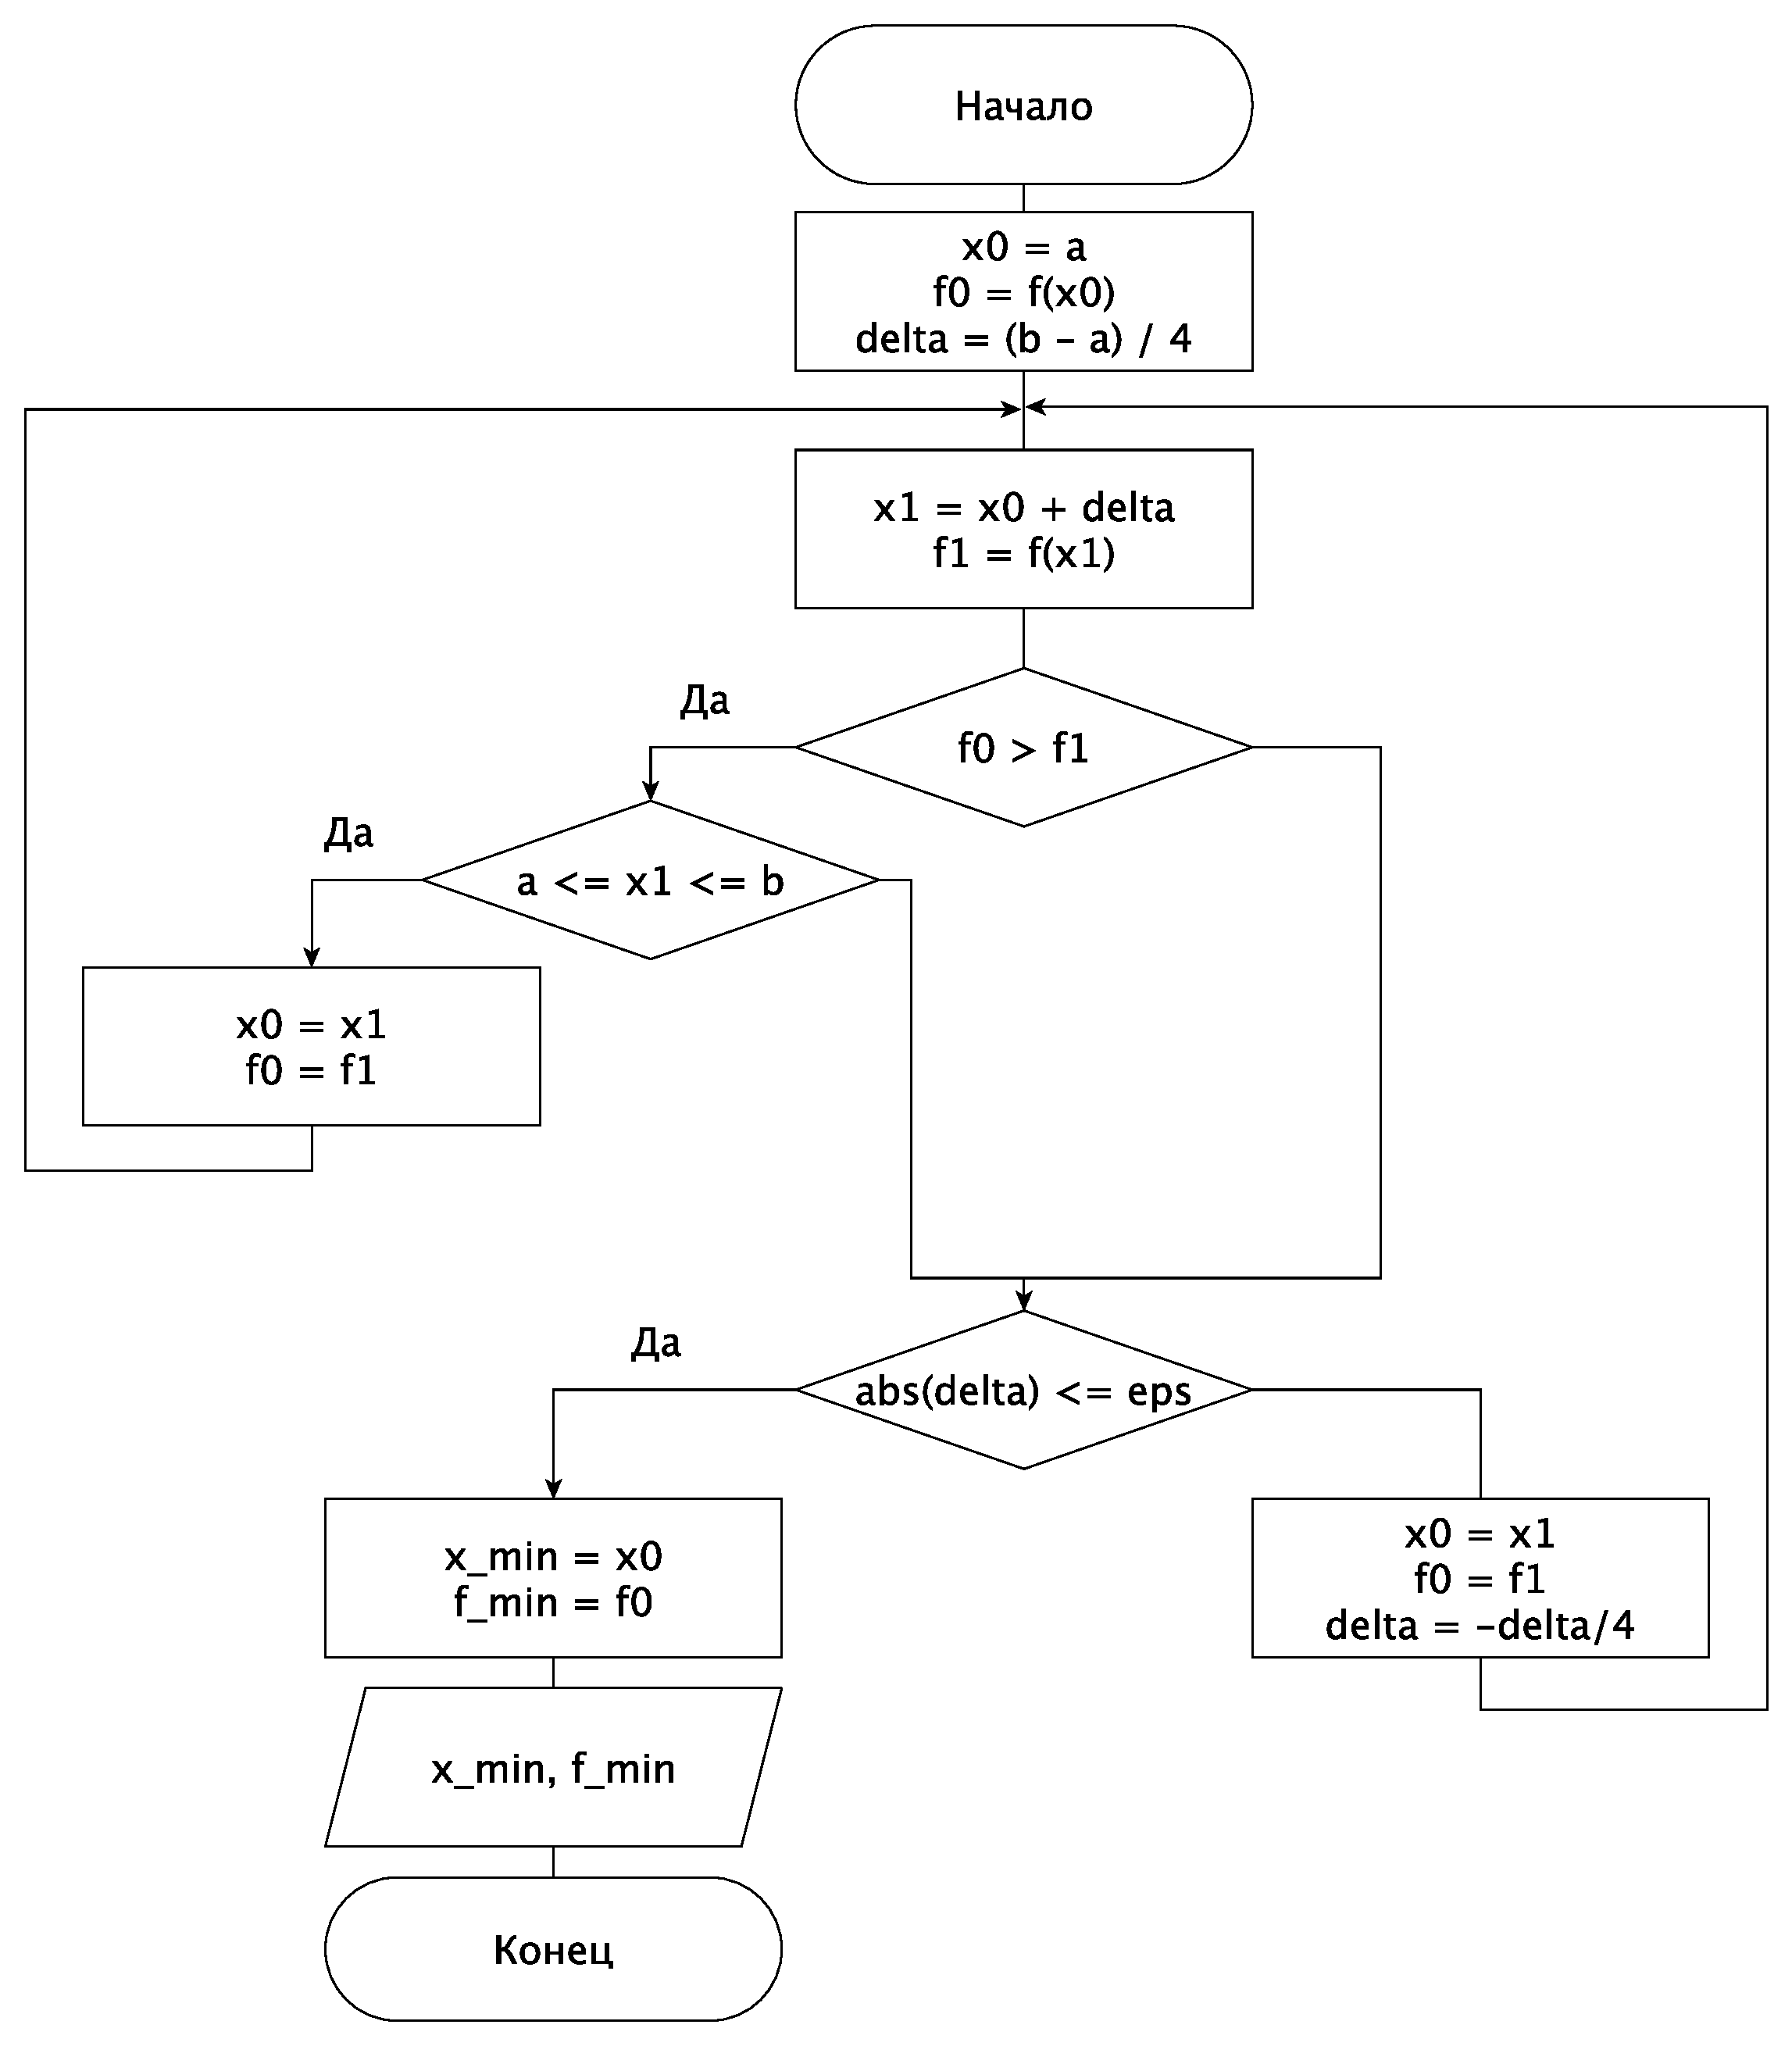
\includegraphics[width=0.7\textwidth]{assets/1.png}
    \caption{Окно работы программы}
    \label{fig:1}
\end{figure}

\newpage

\begin{figure}[ht]
    \centering
    \includegraphics[width=0.7\textwidth]{assets/2.png}
    \caption{Окно работы программы для увеличенного времени обработки первым оператором}
    \label{fig:2}
\end{figure}


% \chapter{Контрольные вопросы}

\section{Какие из следующих множеств регулярны? Для тех, которые регулярны, напишите регулярные выражения}

\begin{enumerate}
	\item Множество цепочек с равным числом нулей и единиц
	
	Не является регулярным.
	
	\item Множество цепочек из {0, 1}* с четным числом нулей и нечетным числом единиц
	
	((0(00)*1)(1(00)*1)*1(00)*01|(0(00)*1)(1(00)*1)*0|0(00)*01|1)
(((10)(00)*1|0)(1(00)*1)*1(00)*01|((10)(00)*1|0)(1(00)*1)*0|(10)(00)*01|11)*

	\item Множество цепочек из {0, 1}*, длины которых делятся на 3
	
	((0|1)(0|1)(0|1))*
	
	\item Множество цепочек из {0, 1}*, не содержащих подцепочки 101
	
	0*(1|00|000)*0*
\end{enumerate}

\section{Найдите праволинейные грамматики для тех множеств из вопроса 1, которые регулярны}

\begin{enumerate}
	\item[2.] Множество цепочек из {0, 1}* с четным числом нулей и нечетным числом единиц
	
	S -> 1C|0A 
	
	A -> 0S|1B
	
	B -> 1A|0C
	
	C -> 1S|0B|$\epsilon$
	
	\item[3.] Множество цепочек из {0, 1}*, длины которых делятся на 3
	
	S -> 0A|1A|$\epsilon$
	
	A -> 0B|1B
	
	B -> 0S|1S
	
	\item[4.] Множество цепочек из {0, 1}*, не содержащих подцепочки 101
	
	S -> 0S|$\epsilon$A
	
	A -> 1A|00A|000A|$\epsilon$B
	
	B -> 0B|$\epsilon$
	
\end{enumerate}

\section{Найдите детерминированные и недетерминированные конечные автоматы для тех множеств из вопроса 1, которые регулярны}

\begin{enumerate}
	\item[2.] Множество цепочек из {0, 1}* с четным числом нулей и нечетным числом единиц
	
	\begin{enumerate}
		\item НКА
		
		\includeimage
    	{nfa_2}
    	{f}
    	{h!}
    	{0.9\textwidth}
    	{НКА}
		
		\item ДКА
		
		\includeimage
    	{dfa_2}
    	{f}
    	{h!}
    	{0.9\textwidth}
    	{ДКА}
		
	\end{enumerate}
	
	\item[3.] Множество цепочек из {0, 1}*, длины которых делятся на 3
	
	\begin{enumerate}
		\item НКА
		
		\includeimage
    	{nfa_3}
    	{f}
    	{h!}
    	{0.9\textwidth}
    	{НКА}
		
		\item ДКА
		
		\includeimage
    	{dfa_3}
    	{f}
    	{h!}
    	{0.9\textwidth}
    	{ДКА}
		
	\end{enumerate}
	
	\item[4.] Множество цепочек из {0, 1}*, не содержащих подцепочки 101
	
	\begin{enumerate}
		\item НКА
		
		\includeimage
    	{nfa_4}
    	{f}
    	{h!}
    	{0.9\textwidth}
    	{НКА}
		
		\item ДКА
		
		\includeimage
    	{dfa_4}
    	{f}
    	{h!}
    	{0.9\textwidth}
    	{ДКА}
		
	\end{enumerate}
	
\end{enumerate}

\section{Найдите конечный автомат с минимальным числом состояний для языка, определяемого автоматом M = (\{A, B, C, D, E\}, \{0, 1\}, d, A, \{E, F\}), где функция задается таблицей}

\newpage

% Please add the following required packages to your document preamble:
% \usepackage{multirow}
\begin{table}[h!]
\caption{}
\label{tab:my-table}
\begin{tabular}{|l|ll|}
\hline
\multirow{2}{*}{\textbf{Состояние}} & \multicolumn{2}{l|}{\textbf{Вход}}           \\ \cline{2-3} 
                                    & \multicolumn{1}{l|}{\textbf{0}} & \textbf{1} \\ \hline
A                                   & \multicolumn{1}{l|}{B}          & C          \\ \hline
B                                   & \multicolumn{1}{l|}{E}          & F          \\ \hline
C                                   & \multicolumn{1}{l|}{A}          & A          \\ \hline
D                                   & \multicolumn{1}{l|}{F}          & E          \\ \hline
E                                   & \multicolumn{1}{l|}{D}          & F          \\ \hline
F                                   & \multicolumn{1}{l|}{D}          & E          \\ \hline
\end{tabular}
\end{table}

Исходный конечный автомат:

\includeimage
    {last_dfa}
    {f}
    {h!}
    {0.9\textwidth}
    {Конечный автомат}

Классы 0-эквивалентности:

\begin{equation*}
\{A, B, C, D\}, \{E, F\}.
\end{equation*}

Классы 1-эквивалентности:

\begin{equation*}
\{A, C\}, \{B, D\}, \{E, F\}.
\end{equation*}

Классы 2-эквивалентности:

\begin{equation*}
\{A\}, \{C\}, \{B, D\}, \{E, F\}.
\end{equation*}

Классы 3-эквивалентности:

\begin{equation*}
\{A\}, \{C\}, \{B, D\}, \{E, F\}.
\end{equation*}

Классы 3-эквивалентности и 2-эквивалентности совпадают. Таким образом, в минимизированном конечном автомате будет 4 состояния:

\begin{equation*}
\{A\}, \{C\}, \{B, D\}, \{E, F\}.
\end{equation*}

Таким образом, минимизированный конечный автомат:

\includeimage
    {last_minimized}
    {f}
    {h!}
    {0.7\textwidth}
    {Минимизированный конечный автомат}

\end{document}